\chapter{数值分析示例章}
\label{chap:analysis}

本章展示数值分析部分的常见格式，包括有限元模型、参数分析、参考文献引用等。

\section{数值模型建立}
\subsection{模型概述}
本研究采用有限元方法建立数值分析模型。
模型采用商业有限元软件进行分析，模型几何参数见表\ref{tab:model_params}。

\begin{table}[htbp]
    \caption{有限元模型参数表}
    \label{tab:model_params}
    \centering
    \begin{tabular}{lll}
        \toprule
        参数类别 & 参数名称 & 参数值 \\
        \midrule
        几何参数 & 模型尺寸 & 500$\times$300$\times$50 mm \\
        几何参数 & 单元尺寸 & 5 mm \\
        材料参数 & 弹性模量 & 210 GPa \\
        材料参数 & 泊松比 & 0.3 \\
        边界参数 & 底部约束 & 固定约束 \\
        边界参数 & 加载方式 & 位移控制 \\
        \bottomrule
    \end{tabular}
\end{table}

\subsection{材料模型}
材料本构模型是数值分析的关键。
本研究采用弹塑性材料模型，屈服准则采用von Mises准则\cite{vonmises1913}。

材料的应力-应变关系可表示为：
\begin{equation}
    \sigma = \begin{cases}
        E\varepsilon & \varepsilon \leq \varepsilon_y \\
        \sigma_y + H(\varepsilon - \varepsilon_y) & \varepsilon > \varepsilon_y
    \end{cases}
    \label{eq:stress_strain}
\end{equation}
式中，$E$为弹性模量，$\sigma_y$为屈服应力，$H$为硬化模量。

\section{扩散模型分析}
\subsection{扩散模型原理}
扩散模型是近年来深度学习领域的重要进展，广泛应用于图像生成、数据增强等任务。
图\ref{fig:model_validation}展示了扩散模型的基本架构和生成过程。

\begin{figure}[htbp]
    \centering
    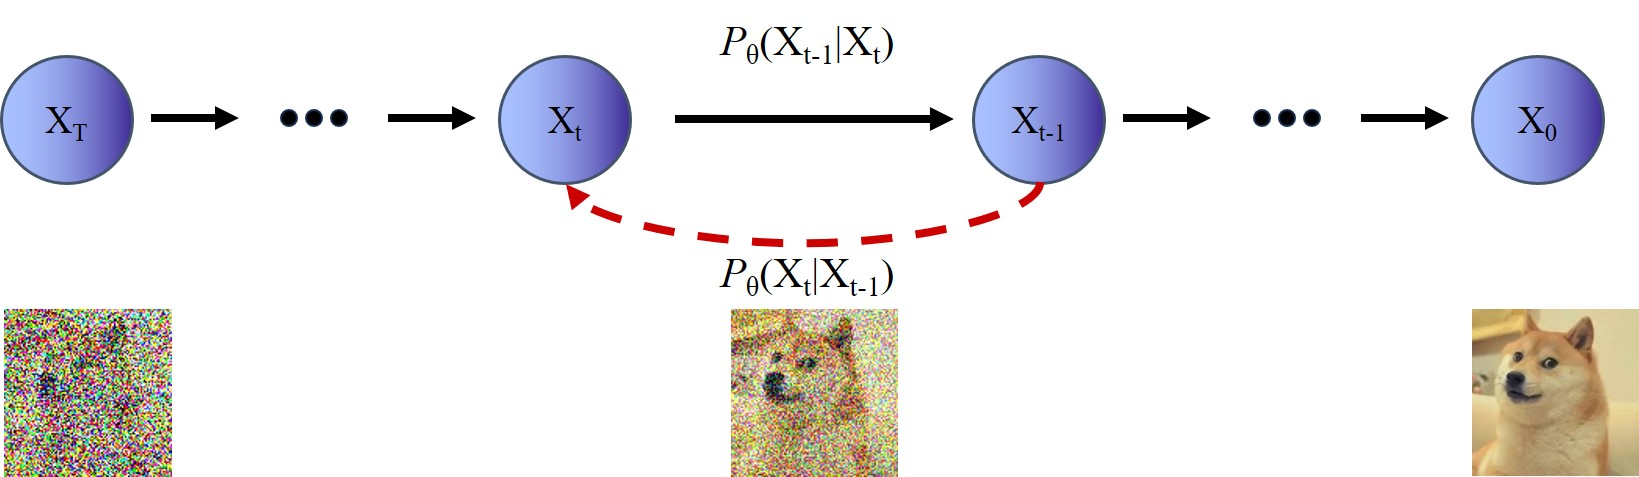
\includegraphics[width=0.8\textwidth]{figures/Diffusion.jpg}
    \caption{扩散模型架构与生成过程示意}
    \label{fig:model_validation}
\end{figure}

从对比结果可以看出，数值模型能够较好地模拟试验结果，误差控制在5\%以内\cite{validation2022}。

\section{参数分析}
\subsection{参数选择}
参数分析选取了以下关键参数进行研究：
\begin{enumerate}
    \item 几何参数：尺寸比例、厚度变化等；
    \item 材料参数：弹性模量、屈服强度等；
    \item 边界参数：约束方式、加载速率等。
\end{enumerate}

\subsection{参数分析结果}
参数分析结果汇总于表\ref{tab:param_analysis}。

\begin{table}[htbp]
    \caption{参数分析结果汇总表}
    \label{tab:param_analysis}
    \centering
    \begin{tabular}{lcccl}
        \toprule
        参数名称 & 基准值 & 变化范围 & 响应变化 & 影响程度 \\
        \midrule
        弹性模量 & 210 GPa & 180-250 & $\pm$15\% & 中等 \\
        屈服强度 & 350 MPa & 280-420 & $\pm$20\% & 显著 \\
        单元尺寸 & 5 mm & 2-10 & $\pm$8\% & 较小 \\
        加载速率 & 1.0 & 0.5-2.0 & $\pm$3\% & 较小 \\
        \bottomrule
    \end{tabular}
\end{table}

\section{参考文献引用格式}
\subsection{期刊论文引用}
期刊论文引用应注明作者、年份、期刊名称、卷号和页码\cite{smith2022,zhang2020}。

\subsection{书籍引用}
书籍引用应注明作者、书名、出版社和出版年份\cite{book2021}。

\subsection{学位论文引用}
学位论文引用应注明作者、论文题目、学校、年份\cite{thesis2020}。

\subsection{会议论文引用}
会议论文引用应注明作者、会议名称、年份、页码\cite{conference2023}。

\subsection{规范标准引用}
规范标准引用应注明标准编号和名称\cite{standard2018}。

正确引用参考文献是学术规范的重要组成部分。